\chapter{ScatterNet Visualization}
\section{Scatternets}\label{ch:scatternets}
% Let us define the pairs of authors here

  Scatternets get their own chapter as they have been a very large influence on
  our work, as well as being quite distinct from the previous discussions on
  learned methods. They were first introduced by  
  \citeauthor{bruna_classification_2011} in their work 
  \citep{bruna_classification_2011}, and then were rigorously defined by Mallat
  in \citep{mallat_group_2012}. Several updates and newer models have since
  been released by Mallat's group, which we will review in this chapter.
  
  It is helpful to introduce this chapter with one further note. Unlike the
  CNNs introduced in \autoref{sec:cnns}, which were set up to minimize some
  cost function which had certain constraints to promote certain properties,
  the scattering operator may be thought of as an operator $\Phi$ which has
  some desirable properties for image understanding. These properties may
  ultimately help us minimize some cost function and improve our image
  understanding system, which we explore more in
  \autoref{ch:scat_deep}.


  \section{Translation Invariant Scatternets}
  The translation invariant Scatternets were mostly covered in
  \citep{bruna_invariant_2013}. This section summarises the method of this
  paper.

  \subsection{Defining the Properties}
  The first release of Scatternets aimed at building a translation invariant
  operator, which was also stable to additive noise and deformations. Translation
  is often defined as being uninformative for classification --- an object
  appearing in the centre of the image should be treated the same way as an
  the same object appearing in the corner of an image, i.e.,\ $\Phi x$ is
  invariant to translations $x_c(\bmu{u}) = x(\bmu{u}-\bmu{c})$\footnote{here
  we adopt a slight variation on \Bruna's notation, by using boldface letters to
  represent vectors, as is the custom in Signal Processing} by 
  $\bmu{c}=(c_1,c_2) \in \mathbb{R}^2$ if
  % The first requirement for Scatternets - translation invariance
  \begin{equation}\label{eq:scat_trans_invariance}
    \Phi x_c = \Phi x
  \end{equation}

  Stability to additive noise is another good choice to include in this operator,
  as it is a common feature in measured signals. Stability is defined in terms of
  Lipschitz continuity, which is a strong form of uniform continuity for
  functions, which we briefly introduce here.

  Formally, a Lipschitz continuous function is limited in how fast it can change;
  there exists an upper bound on the gradient the function can take, although it
  doesn't necessarily need to be differentiable everywhere. The modulus operator
  $|x|$ is a good example of a function that has a bounded derivative and so is
  Lipschitz continuous, but isn't differentiable everywhere.

  \begin{figure}
    \begin{center}
      % 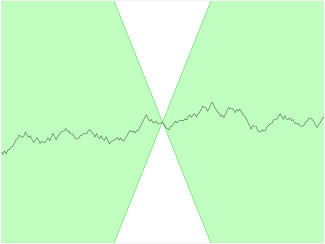
\includegraphics[scale=0.8]{images/Lipschitz_continuity.png}
      \caption[A Lipschitz continuous function]
              {A Lipschitz continuous function is shown. There is a cone for this
              function (shown in white) such that the graph always remains entirely outside
              the cone as it's shifted across. The minimum gradient needed for this to hold
              is called the `best Lipschitz constant'.}
      \label{fig:lipschitz}
    \end{center}
  \end{figure}

  Returning again to stability to additive noise, \Bruna\ state that for a new
  signal $x'(\bmu{u}) = x(\bmu{u}) + \epsilon(\bmu{u})$, there must exist
  a bounded $C>0$ s.t.
  % The second requirement - noise stability
  \begin{equation}\label{eq:scat_noise_stability}
    \|\Phi x' - \Phi x\| \leq C \|x' - x\|
  \end{equation}
  The final requirement is to be stable to small deformations. Enough so that we
  can ignore intra-class variations, but not so invariant that an object can
  morph into another (in the case of MNIST for example, we do not want to be so
  stable to deformations that 7s can map to 1s). Formally, for a new signal
  $x_{\tau}(\bmu{u}) = x(\bmu{u}-\tau(\bmu{u}))$, where $\tau(\bmu{u})$ is a non
  constant displacement field (i.e.,\ not just a translation) that deforms the
  image, we require a $C>0$ s.t.
  % The third requirement - deformation stability
  \protect\begin{equation}\label{eq:scat_deformation_stability}
    \|\Phi x_{\tau} - \Phi x \| \leq C \|x\| \sup_{\bmu{u}} |\nabla\tau(\bmu{u})|
  \protect\end{equation}
  The term on the right $|\nabla\tau(\bmu{u})|$ measures the deformation
  amplitude, so the supremum of it is a limit on the global defomation amplitude.

\subsection{Finding the Right Operator}
  A Fourier modulus satisfies the first two of these requirements, in that it is
  both translation invariant and stable to additive noise, but it is unstable to
  deformations due to the infinite support of the sinusoid basis functions it
  uses. It also loses too much information --- very different signals can all
  have the same Fourier modulus, e.g.\ a chirp, white noise and the Dirac delta
  function all have flat spectra.

  Unlike the Fourier modulus, a wavelet transform
  is stable to deformations due to the grouping together frequencies into dyadic
  packets \citep{mallat_group_2012}, however, the wavelet transform is not invariant to
  shifts. 
  
  We saw in \autoref{ch:freq_analysis} that the modulus of complex, analytic
  wavelets commuted with shifts. The real and imaginary parts are also
  commutative with shifts, but these vary much quicker than the modulus
  (\autoref{fig:pulse_response}).  Interestingly, the modulus operator, in this
  case, does not lose any information \citep{waldspurger_phase_2012} (due to the
  redundancies of the wavelet transform), which is why it may be nice to think
  of it as a \emph{demodulator}.

  \begin{figure}
    \begin{center}
      \newlength\figureheight 
      \newlength\figurewidth 
      \setlength\figureheight{6cm} 
      \setlength\figurewidth{8cm}
      % % This file was created by matlab2tikz.
%
%The latest updates can be retrieved from
%  http://www.mathworks.com/matlabcentral/fileexchange/22022-matlab2tikz-matlab2tikz
%where you can also make suggestions and rate matlab2tikz.
%
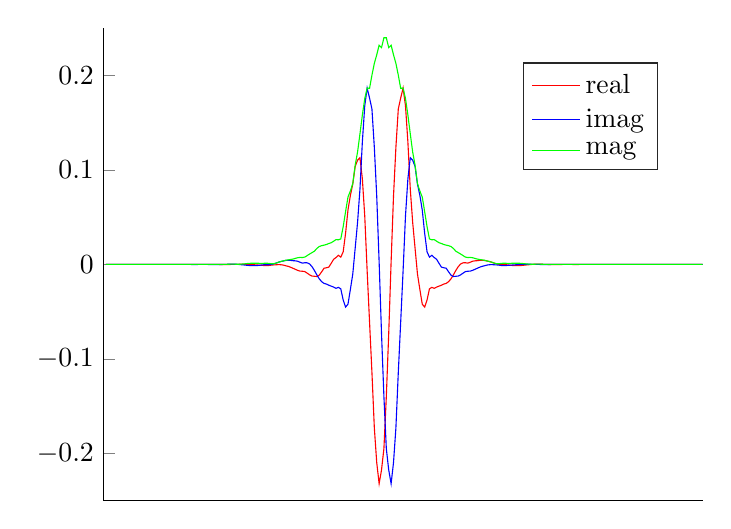
\begin{tikzpicture}

\begin{axis}[%
width=0.951\figurewidth,
height=\figureheight,
at={(0\figurewidth,0\figureheight)},
scale only axis,
xmin=0,
xmax=250,
xtick={\empty},
ymin=-0.25,
ymax=0.25,
axis background/.style={fill=white},
axis x line*=bottom,
axis y line*=left,
legend style={at={(0.7,0.7)},anchor=south west,legend cell align=left,align=left,draw=white!15!black}
]
\addplot [color=red,solid]
  table[row sep=crcr]{%
1	0\\
2	0\\
3	0\\
4	0\\
5	0\\
6	0\\
7	0\\
8	0\\
9	0\\
10	0\\
11	0\\
12	0\\
13	0\\
14	0\\
15	0\\
16	0\\
17	0\\
18	0\\
19	3.40598214094164e-12\\
20	0\\
21	-6.87793140105386e-11\\
22	-9.08261904251105e-11\\
23	4.62741351914918e-10\\
24	1.258882500922e-09\\
25	-3.90768164174049e-09\\
26	-4.94207941791755e-09\\
27	2.25257324923178e-08\\
28	4.47997487754667e-08\\
29	-3.72860948552819e-08\\
30	-7.72685694491778e-08\\
31	1.74091939763211e-07\\
32	3.20701693438365e-07\\
33	6.69906724002732e-08\\
34	-2.57334712035421e-07\\
35	-7.60438752193682e-07\\
36	-6.79175261479185e-07\\
37	3.85670908249705e-07\\
38	1.95760682064202e-06\\
39	2.70916484936271e-06\\
40	3.70985229264904e-06\\
41	5.60263903783335e-06\\
42	7.15200536225569e-06\\
43	9.42804407054984e-06\\
44	9.19816726897712e-06\\
45	4.09312377588624e-06\\
46	-2.18677142696421e-06\\
47	-7.78276608370347e-07\\
48	-2.49334758811333e-06\\
49	-1.24876312688003e-05\\
50	-2.40789294574741e-05\\
51	-5.00285382615212e-05\\
52	-5.19808121979403e-05\\
53	-8.56826227144868e-06\\
54	5.38557733758203e-05\\
55	9.09976831863687e-05\\
56	0.000118256932396166\\
57	0.000164847396440429\\
58	0.000172590561244501\\
59	0.000156541159523113\\
60	7.26324581485654e-05\\
61	-4.32251690266487e-05\\
62	-0.000209156467228341\\
63	-0.000355191843470207\\
64	-0.000528083903626197\\
65	-0.000723523151351148\\
66	-0.000904822353516488\\
67	-0.00117977622340421\\
68	-0.00127386800702199\\
69	-0.00107595626030387\\
70	-0.000731388490979029\\
71	-0.000492950213440953\\
72	-0.000355077529547522\\
73	-0.000176866907141536\\
74	-0.000304238537971187\\
75	-0.000669112865679403\\
76	-0.00137639751374934\\
77	-0.0019999871515232\\
78	-0.00288266647428663\\
79	-0.00399474325488351\\
80	-0.0051470769192401\\
81	-0.00623242432359724\\
82	-0.00706986688887293\\
83	-0.00719378257668194\\
84	-0.00758143497956961\\
85	-0.00925240669242568\\
86	-0.0110384455473666\\
87	-0.0122898662832043\\
88	-0.0125276118821436\\
89	-0.0127859505897159\\
90	-0.0113952391112889\\
91	-0.00784660452604257\\
92	-0.00401960851433002\\
93	-0.00350870901525763\\
94	-0.00282836192466074\\
95	0.00117836761234312\\
96	0.00541190932558586\\
97	0.00731202945632788\\
98	0.00961314726741875\\
99	0.00773250299419411\\
100	0.013341034228591\\
101	0.0329962818862013\\
102	0.0576135809313121\\
103	0.0730546535876305\\
104	0.084986015392322\\
105	0.103631123640744\\
106	0.110327196614011\\
107	0.112909993173503\\
108	0.0905813378752889\\
109	0.0513323912871931\\
110	-0.00674939368285724\\
111	-0.060713087095648\\
112	-0.114305418494503\\
113	-0.17300702433579\\
114	-0.209749288098405\\
115	-0.231992927271329\\
116	-0.217464614066301\\
117	-0.194784442562913\\
118	-0.140070485832163\\
119	-0.0733218645827401\\
120	0.00256331681737184\\
121	0.0722909879534431\\
122	0.123938750062336\\
123	0.164537100743611\\
124	0.1761522691017\\
125	0.186614921947609\\
126	0.16786851431561\\
127	0.129648576703118\\
128	0.0797149042875755\\
129	0.0445213447780424\\
130	0.0170433369608732\\
131	-0.0101767458153209\\
132	-0.0264788340863422\\
133	-0.0420467635360721\\
134	-0.0451140888775753\\
135	-0.0376649209952693\\
136	-0.0258341146252317\\
137	-0.0242550663754605\\
138	-0.0252504924158299\\
139	-0.0239210066309461\\
140	-0.0229612977291479\\
141	-0.0220048369351539\\
142	-0.0207817770698637\\
143	-0.0200383376462408\\
144	-0.0182129976759503\\
145	-0.0151705843558306\\
146	-0.0110133286799118\\
147	-0.00640572486704498\\
148	-0.00241914987168933\\
149	0.000501553892557113\\
150	0.00171502644229679\\
151	0.00182682703744143\\
152	0.00135819388712596\\
153	0.0023202015883891\\
154	0.00338143714657009\\
155	0.0038167928839548\\
156	0.00398922920965832\\
157	0.00435012390937784\\
158	0.00438744590069432\\
159	0.00420434222714658\\
160	0.00365909375507545\\
161	0.0031096699498426\\
162	0.00234243116660081\\
163	0.00139821952573963\\
164	0.000556075684303888\\
165	-5.51706115206466e-05\\
166	-0.000331691562229006\\
167	-0.000361308885120112\\
168	-0.00030880647995183\\
169	-0.000606048853947934\\
170	-0.000942240424391602\\
171	-0.00116480277977496\\
172	-0.00125325781851377\\
173	-0.00129181029001784\\
174	-0.00115716277061801\\
175	-0.000949777311562008\\
176	-0.000655071283282308\\
177	-0.000401238951280002\\
178	-0.000168066677392165\\
179	7.51939646498624e-05\\
180	0.000224400979048634\\
181	0.000325006343811925\\
182	0.00029951693903595\\
183	0.000193407642771761\\
184	5.23403692689068e-05\\
185	-7.08866952670796e-07\\
186	-1.49391620378925e-05\\
187	-3.63681852437294e-05\\
188	-3.66387543450729e-05\\
189	-4.31719371365099e-05\\
190	-3.68830397411496e-05\\
191	-1.45273881114298e-05\\
192	7.69634724727019e-06\\
193	1.40718734743013e-05\\
194	9.47996727945057e-06\\
195	1.08877455419357e-06\\
196	-8.37952554555356e-06\\
197	-9.54752048564336e-06\\
198	-6.25889587127397e-06\\
199	-2.89688757013566e-06\\
200	7.1722847502998e-07\\
201	1.69289428040498e-06\\
202	1.08252608403094e-06\\
203	5.10006804932853e-07\\
204	-3.13462849361191e-07\\
205	-3.54749535554903e-07\\
206	-1.07355897601877e-07\\
207	-3.86544340676565e-08\\
208	4.33594828396285e-08\\
209	5.64209933272261e-08\\
210	2.65249108795441e-08\\
211	1.4160405157173e-08\\
212	-9.40796883785182e-10\\
213	-2.76659516509318e-09\\
214	1.45966616149977e-09\\
215	3.51734339084897e-10\\
216	-1.27226347003132e-10\\
217	-8.49537384694854e-11\\
218	0\\
219	4.77098801261746e-12\\
220	0\\
221	0\\
222	0\\
223	0\\
224	0\\
225	0\\
226	0\\
227	0\\
228	0\\
229	0\\
230	0\\
231	0\\
232	0\\
233	0\\
234	0\\
235	0\\
236	0\\
237	0\\
238	0\\
239	0\\
240	0\\
241	0\\
242	0\\
243	0\\
244	0\\
245	0\\
246	0\\
247	0\\
248	0\\
249	0\\
250	0\\
};
\addlegendentry{real};

\addplot [color=blue,solid]
  table[row sep=crcr]{%
1	0\\
2	0\\
3	0\\
4	0\\
5	0\\
6	0\\
7	0\\
8	0\\
9	0\\
10	0\\
11	0\\
12	0\\
13	0\\
14	0\\
15	0\\
16	4.77098801261746e-12\\
17	0\\
18	-8.49537384694854e-11\\
19	-1.27226347003132e-10\\
20	3.51734339084897e-10\\
21	1.45966616149977e-09\\
22	-2.76659516509318e-09\\
23	-9.40796883785182e-10\\
24	1.4160405157173e-08\\
25	2.65249108795441e-08\\
26	5.64209933272261e-08\\
27	4.33594828396285e-08\\
28	-3.86544340676565e-08\\
29	-1.07355897601877e-07\\
30	-3.54749535554903e-07\\
31	-3.13462849361191e-07\\
32	5.10006804932853e-07\\
33	1.08252608403094e-06\\
34	1.69289428040498e-06\\
35	7.1722847502998e-07\\
36	-2.89688757013566e-06\\
37	-6.25889587127397e-06\\
38	-9.54752048564336e-06\\
39	-8.37952554555356e-06\\
40	1.08877455419357e-06\\
41	9.47996727945057e-06\\
42	1.40718734743013e-05\\
43	7.69634724727019e-06\\
44	-1.45273881114298e-05\\
45	-3.68830397411496e-05\\
46	-4.31719371365099e-05\\
47	-3.66387543450729e-05\\
48	-3.63681852437294e-05\\
49	-1.49391620378925e-05\\
50	-7.08866952670774e-07\\
51	5.23403692689068e-05\\
52	0.000193407642771761\\
53	0.00029951693903595\\
54	0.000325006343811925\\
55	0.000224400979048634\\
56	7.51939646498624e-05\\
57	-0.000168066677392165\\
58	-0.000401238951280002\\
59	-0.000655071283282308\\
60	-0.000949777311562008\\
61	-0.00115716277061801\\
62	-0.00129181029001784\\
63	-0.00125325781851377\\
64	-0.00116480277977496\\
65	-0.000942240424391602\\
66	-0.000606048853947934\\
67	-0.00030880647995183\\
68	-0.000361308885120112\\
69	-0.000331691562229006\\
70	-5.51706115206467e-05\\
71	0.000556075684303888\\
72	0.00139821952573963\\
73	0.00234243116660081\\
74	0.0031096699498426\\
75	0.00365909375507545\\
76	0.00420434222714658\\
77	0.00438744590069432\\
78	0.00435012390937784\\
79	0.00398922920965832\\
80	0.0038167928839548\\
81	0.00338143714657009\\
82	0.0023202015883891\\
83	0.00135819388712596\\
84	0.00182682703744143\\
85	0.0017150264422968\\
86	0.000501553892557114\\
87	-0.00241914987168932\\
88	-0.00640572486704498\\
89	-0.0110133286799118\\
90	-0.0151705843558306\\
91	-0.0182129976759503\\
92	-0.0200383376462408\\
93	-0.0207817770698637\\
94	-0.0220048369351539\\
95	-0.0229612977291479\\
96	-0.0239210066309461\\
97	-0.0252504924158299\\
98	-0.0242550663754605\\
99	-0.0258341146252317\\
100	-0.0376649209952693\\
101	-0.0451140888775753\\
102	-0.0420467635360721\\
103	-0.0264788340863422\\
104	-0.0101767458153209\\
105	0.0170433369608732\\
106	0.0445213447780424\\
107	0.0797149042875755\\
108	0.129648576703118\\
109	0.16786851431561\\
110	0.186614921947609\\
111	0.1761522691017\\
112	0.164537100743611\\
113	0.123938750062336\\
114	0.0722909879534431\\
115	0.00256331681737185\\
116	-0.0733218645827401\\
117	-0.140070485832163\\
118	-0.194784442562913\\
119	-0.217464614066301\\
120	-0.231992927271329\\
121	-0.209749288098405\\
122	-0.17300702433579\\
123	-0.114305418494503\\
124	-0.0607130870956479\\
125	-0.00674939368285723\\
126	0.0513323912871931\\
127	0.0905813378752889\\
128	0.112909993173503\\
129	0.110327196614011\\
130	0.103631123640744\\
131	0.0849860153923221\\
132	0.0730546535876306\\
133	0.0576135809313121\\
134	0.0329962818862013\\
135	0.013341034228591\\
136	0.00773250299419411\\
137	0.00961314726741875\\
138	0.00731202945632788\\
139	0.00541190932558586\\
140	0.00117836761234312\\
141	-0.00282836192466074\\
142	-0.00350870901525763\\
143	-0.00401960851433002\\
144	-0.00784660452604257\\
145	-0.0113952391112889\\
146	-0.0127859505897159\\
147	-0.0125276118821436\\
148	-0.0122898662832043\\
149	-0.0110384455473666\\
150	-0.00925240669242567\\
151	-0.00758143497956961\\
152	-0.00719378257668194\\
153	-0.00706986688887293\\
154	-0.00623242432359725\\
155	-0.00514707691924009\\
156	-0.00399474325488351\\
157	-0.00288266647428663\\
158	-0.0019999871515232\\
159	-0.00137639751374934\\
160	-0.000669112865679403\\
161	-0.000304238537971186\\
162	-0.000176866907141536\\
163	-0.000355077529547522\\
164	-0.000492950213440953\\
165	-0.000731388490979029\\
166	-0.00107595626030387\\
167	-0.00127386800702199\\
168	-0.00117977622340421\\
169	-0.000904822353516488\\
170	-0.000723523151351148\\
171	-0.000528083903626196\\
172	-0.000355191843470207\\
173	-0.000209156467228341\\
174	-4.32251690266487e-05\\
175	7.26324581485654e-05\\
176	0.000156541159523113\\
177	0.000172590561244501\\
178	0.000164847396440429\\
179	0.000118256932396166\\
180	9.09976831863687e-05\\
181	5.38557733758203e-05\\
182	-8.56826227144868e-06\\
183	-5.19808121979403e-05\\
184	-5.00285382615212e-05\\
185	-2.40789294574741e-05\\
186	-1.24876312688003e-05\\
187	-2.49334758811333e-06\\
188	-7.78276608370347e-07\\
189	-2.18677142696421e-06\\
190	4.09312377588625e-06\\
191	9.19816726897713e-06\\
192	9.42804407054984e-06\\
193	7.15200536225569e-06\\
194	5.60263903783335e-06\\
195	3.70985229264904e-06\\
196	2.70916484936271e-06\\
197	1.95760682064202e-06\\
198	3.85670908249705e-07\\
199	-6.79175261479185e-07\\
200	-7.60438752193682e-07\\
201	-2.57334712035421e-07\\
202	6.69906724002732e-08\\
203	3.20701693438365e-07\\
204	1.74091939763211e-07\\
205	-7.72685694491778e-08\\
206	-3.72860948552819e-08\\
207	4.47997487754667e-08\\
208	2.25257324923178e-08\\
209	-4.94207941791755e-09\\
210	-3.90768164174049e-09\\
211	1.258882500922e-09\\
212	4.62741351914918e-10\\
213	-9.08261904251105e-11\\
214	-6.87793140105386e-11\\
215	0\\
216	3.40598214094164e-12\\
217	0\\
218	0\\
219	0\\
220	0\\
221	0\\
222	0\\
223	0\\
224	0\\
225	0\\
226	0\\
227	0\\
228	0\\
229	0\\
230	0\\
231	0\\
232	0\\
233	0\\
234	0\\
235	0\\
236	0\\
237	0\\
238	0\\
239	0\\
240	0\\
241	0\\
242	0\\
243	0\\
244	0\\
245	0\\
246	0\\
247	0\\
248	0\\
249	0\\
250	0\\
};
\addlegendentry{imag};

\addplot [color=green,solid]
  table[row sep=crcr]{%
1	0\\
2	0\\
3	0\\
4	0\\
5	0\\
6	0\\
7	0\\
8	0\\
9	0\\
10	0\\
11	0\\
12	0\\
13	0\\
14	0\\
15	0\\
16	4.77098801261746e-12\\
17	0\\
18	8.49537384694854e-11\\
19	1.27271929686423e-10\\
20	3.51734339084897e-10\\
21	1.46128570001326e-09\\
22	2.76808565698103e-09\\
23	1.04844090692416e-09\\
24	1.42162533519356e-08\\
25	2.6811207973177e-08\\
26	5.66370253191664e-08\\
27	4.88615736180845e-08\\
28	5.91707931621314e-08\\
29	1.13646564485961e-07\\
30	3.6306702521868e-07\\
31	3.5856235360137e-07\\
32	6.02458726596314e-07\\
33	1.08459691719828e-06\\
34	1.7123411455216e-06\\
35	1.04531515880701e-06\\
36	2.97543889700524e-06\\
37	6.27076706447628e-06\\
38	9.74614651480286e-06\\
39	8.80658972302032e-06\\
40	3.86632048117235e-06\\
41	1.1011782045051e-05\\
42	1.57850816842511e-05\\
43	1.21705289920691e-05\\
44	1.71945132658123e-05\\
45	3.71094635206701e-05\\
46	4.32272845017189e-05\\
47	3.66470194482135e-05\\
48	3.64535551094453e-05\\
49	1.9470991168914e-05\\
50	2.40893614729532e-05\\
51	7.24042049593117e-05\\
52	0.00020027111903439\\
53	0.000299639469843039\\
54	0.000329438261050387\\
55	0.000242149494617008\\
56	0.000140138625580231\\
57	0.000235416805183551\\
58	0.000436783925820271\\
59	0.000673515791059104\\
60	0.000952550479258007\\
61	0.00115796981521183\\
62	0.00130863297114945\\
63	0.00130261905610722\\
64	0.0012789206875489\\
65	0.00118798264629529\\
66	0.00108903567654817\\
67	0.00121952178306504\\
68	0.00132411623726202\\
69	0.00112592236257258\\
70	0.00073346637353879\\
71	0.000743115118676452\\
72	0.00144260108628446\\
73	0.00234909890662455\\
74	0.00312451728830885\\
75	0.00371976869381013\\
76	0.0044239081905961\\
77	0.00482178702741808\\
78	0.00521855765790864\\
79	0.00564552241689185\\
80	0.00640783182766075\\
81	0.00709064384421969\\
82	0.007440857023028\\
83	0.0073208741551538\\
84	0.0077984263396001\\
85	0.00941001303398782\\
86	0.0110498342254224\\
87	0.0125256975598461\\
88	0.01407033654686\\
89	0.0168752464009988\\
90	0.0189736159996144\\
91	0.0198313511121225\\
92	0.0204375201096715\\
93	0.0210758937446378\\
94	0.0221858621585816\\
95	0.0229915146007476\\
96	0.024525564637458\\
97	0.026287889645464\\
98	0.0260906275367817\\
99	0.0269665177771404\\
100	0.0399578461365013\\
101	0.0558930732163425\\
102	0.0713249958400785\\
103	0.0777052833813811\\
104	0.0855931595844764\\
105	0.105023259908484\\
106	0.118971595154272\\
107	0.138214082220365\\
108	0.158157302115399\\
109	0.17554159761661\\
110	0.186736936380028\\
111	0.186321498637064\\
112	0.200345167693949\\
113	0.212819745880261\\
114	0.221857501106166\\
115	0.232007088031867\\
116	0.229492819488748\\
117	0.239918152847597\\
118	0.239918152847597\\
119	0.229492819488748\\
120	0.232007088031867\\
121	0.221857501106166\\
122	0.212819745880261\\
123	0.200345167693949\\
124	0.186321498637064\\
125	0.186736936380028\\
126	0.17554159761661\\
127	0.158157302115399\\
128	0.138214082220365\\
129	0.118971595154272\\
130	0.105023259908484\\
131	0.0855931595844765\\
132	0.0777052833813811\\
133	0.0713249958400785\\
134	0.0558930732163425\\
135	0.0399578461365013\\
136	0.0269665177771404\\
137	0.0260906275367817\\
138	0.026287889645464\\
139	0.024525564637458\\
140	0.0229915146007476\\
141	0.0221858621585816\\
142	0.0210758937446378\\
143	0.0204375201096715\\
144	0.0198313511121225\\
145	0.0189736159996144\\
146	0.0168752464009988\\
147	0.01407033654686\\
148	0.0125256975598461\\
149	0.0110498342254224\\
150	0.00941001303398781\\
151	0.0077984263396001\\
152	0.00732087415515381\\
153	0.007440857023028\\
154	0.0070906438442197\\
155	0.00640783182766075\\
156	0.00564552241689185\\
157	0.00521855765790864\\
158	0.00482178702741808\\
159	0.0044239081905961\\
160	0.00371976869381013\\
161	0.00312451728830885\\
162	0.00234909890662455\\
163	0.00144260108628446\\
164	0.000743115118676453\\
165	0.00073346637353879\\
166	0.00112592236257258\\
167	0.00132411623726202\\
168	0.00121952178306504\\
169	0.00108903567654817\\
170	0.00118798264629529\\
171	0.0012789206875489\\
172	0.00130261905610722\\
173	0.00130863297114945\\
174	0.00115796981521183\\
175	0.000952550479258007\\
176	0.000673515791059104\\
177	0.000436783925820271\\
178	0.000235416805183551\\
179	0.000140138625580231\\
180	0.000242149494617008\\
181	0.000329438261050387\\
182	0.000299639469843039\\
183	0.00020027111903439\\
184	7.24042049593117e-05\\
185	2.40893614729532e-05\\
186	1.9470991168914e-05\\
187	3.64535551094453e-05\\
188	3.66470194482135e-05\\
189	4.32272845017189e-05\\
190	3.71094635206701e-05\\
191	1.71945132658123e-05\\
192	1.21705289920691e-05\\
193	1.57850816842511e-05\\
194	1.1011782045051e-05\\
195	3.86632048117234e-06\\
196	8.80658972302032e-06\\
197	9.74614651480286e-06\\
198	6.27076706447628e-06\\
199	2.97543889700524e-06\\
200	1.04531515880701e-06\\
201	1.7123411455216e-06\\
202	1.08459691719828e-06\\
203	6.02458726596314e-07\\
204	3.5856235360137e-07\\
205	3.6306702521868e-07\\
206	1.13646564485961e-07\\
207	5.91707931621314e-08\\
208	4.88615736180845e-08\\
209	5.66370253191664e-08\\
210	2.6811207973177e-08\\
211	1.42162533519356e-08\\
212	1.04844090692416e-09\\
213	2.76808565698103e-09\\
214	1.46128570001326e-09\\
215	3.51734339084897e-10\\
216	1.27271929686423e-10\\
217	8.49537384694854e-11\\
218	0\\
219	4.77098801261746e-12\\
220	0\\
221	0\\
222	0\\
223	0\\
224	0\\
225	0\\
226	0\\
227	0\\
228	0\\
229	0\\
230	0\\
231	0\\
232	0\\
233	0\\
234	0\\
235	0\\
236	0\\
237	0\\
238	0\\
239	0\\
240	0\\
241	0\\
242	0\\
243	0\\
244	0\\
245	0\\
246	0\\
247	0\\
248	0\\
249	0\\
250	0\\
};
\addlegendentry{mag};

\end{axis}
\end{tikzpicture}% 
      \caption{Real, Imaginary and Modulus of complex wavelet convolved with
               an impulse.}
      \label{fig:pulse_response}
    \end{center}
  \end{figure}
  

  % A tikz diagram to draw what the operator looks like so far
  %\input{tikz/invariant}

  The modulus can be made fully invariant by integrating, i.e.,:
  $$\int F x(\bmu{u})d\bmu{u}= \int | x \ast \psi_{\lambda}(\bmu{u})| d\bmu{u}$$
  is translation invariant. 
  Total invariance to shifts means integrating over the entire function, which
  may not be ideal as it loses a significant amount of information in doing this. Instead
  \citeauthor{bruna_invariant_2013} define scales $2^J$, over which their operator
  is invariant to shifts. Now instead of integrating, the output $\|x \ast \psi_{\lambda}\|$ is
  convolved with an averaging window, or conveniently, the scaling function for
  the chosen wavelet:
  $$\phi_{2^J}(\bmu{u}) = 2^{-2J}\phi(2^{-J}\bmu{u})$$

  Even still, this averaging means that a lot of information is lost from the
  first layer outputs ($\|x \ast \psi_{\lambda}\|$).
  \citeauthor{bruna_invariant_2013} combat this by also convolving the output
  with wavelets that cover the rest of the frequency space, giving  
  $$U[p]x = U[\lambda_2]U[\lambda_1]x = \| | x \ast \psi_{\lambda_1}| 
    \ast \psi_{\lambda_2} \|$$
  The choice of wavelet functions $\lambda_{1}$ and $\lambda_{2}$ is combined
  into a path variable, $p = (\lambda_1, \lambda_2, \ldots \lambda{m})$.

  Local invariants can be again computed by convolving this with another scaling
  function $\phi$. The result is now a multiscale scattering transform, with
  coefficients:
  $$ S[p]x = U[p]x \ast \phi_{2^J}(\bmu{u}) $$
  A graphical representation of this is shown in
  \autoref{fig:scatternet_mallat}.

  \begin{figure}
    \centering
      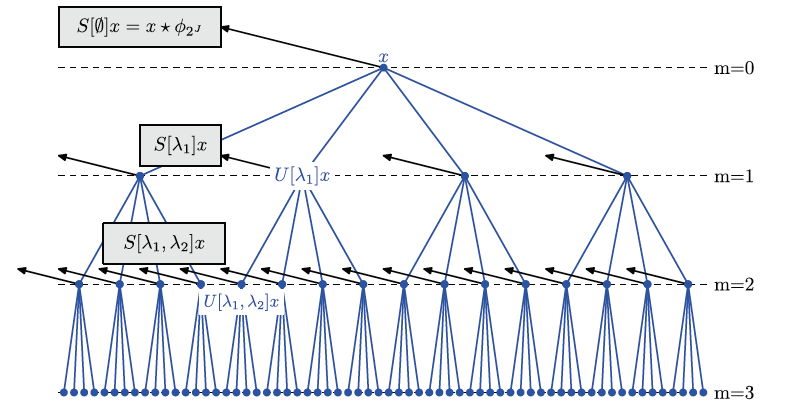
\includegraphics[width=\textwidth]{images/scatternet_diagram.png}
      \caption[Translation Invariant Scatternet Layout]
              {The translation invariant Scattering Transform. Scattering outputs
               are the leftward pointing arrows $S[p]x$, and the intermediate 
               coefficients $U[p]x$ are the centre nodes of the tree. Taken
               from \citep{bruna_invariant_2013}.}
      \label{fig:scatternet_mallat}
  \end{figure}

  % \begin{eqnarray*}
  % \bm{lambda} &=& (j, \theta)
  % % Scattering transform equation
  % \begin{eqnarray*}
  % \Phi x & = & \{S[\bmu{p}]x(\bmu{u}) | \bmu{p} = (\bmu{\lambda_{1}},
  % \bmu{\lambda_{2}}, \ldots \bmu{\lambda_{m}})

\section{Rotation and Translation Invariant Scatternets}
  Mallat's group refined their Scatternet architecture by expanding their list
  of invariants to also include rotation. They also experimented with adding
  scale invariance in \citep{sifre_rotation_2013}, but it was limited to only
  averaging over scale once, and they were no longer using
  it in \citep{oyallon_deep_2015}, so for brevity we omit it. 
  
  This work was done by two authors, each tackling different
  challenges. The first is texture analysis with Sifre in
  \citep{sifre_combined_2012, sifre_rotation_2013, sifre_rigid-motion_2014,
  sifre_rigid-motion_2014-1}, and the second is image classification with
  Oyallon in \citep{oyallon_generic_2013, oyallon_deep_2015}. In this section,
  we outline the properties and structure of this extended Scatternet.

\subsection{An Important note on Joint vs. Separable Invariants}
  When building multiple invariants, some thought must be given as to how to
  combine them --- separably or jointly? Let us call the group of operations we
  want to be invariant to $G$, with $g \in G$ a single realization from this
  group --- in this case, $G$ is the group of affine transformations. We want
  our operator $\Phi$ to be invariant to all  $g \in G$, i.e.,\ $\Phi(gx)
  = \Phi(x)$. Building separable invariants would mean representing the group
  as $G=G_2G_1$ (an assumption of the group, not of our model), and building
  $\Phi = \Phi_2 \Phi_1$, where $\Phi_1$ is invariant to members of $G_1$ and
  covariant to members of $G_2$, and $\Phi_2$ is invariant to members of $G_2$.
  I.e.,\
  \begin{equation}
    \Phi_2(\Phi_1(g_1g_2x)) = \Phi_2(g_2\Phi_1(x)) = \Phi_2(\Phi_1(x))
  \end{equation}
  An example of this would be in the group $G$ of 2D translations, building
  horizontal invariance first, then building vertical invariance second.
  \Bruna\ warn about this approach, however, as it cannot capture the action
  of $G_2$ relative to $G_1$. In the case of veritcal and horizontal
  translations, for example, it would not be able to distinguish if the
  patterns had moved apart as well as being shifted, whereas a joint
  horizontal and vertical translation invariant would be able to distinguish
  these two cases.

  % \begin{figure}[t!]
    % \centering
  % %    \captionsetup[subfigure]{width=0.3\textwdith}
      % \subfloat[]{\includegraphics[width=0.3\textwidth]{scripts/separable_invariance_1.png}
                  % \label{fig:joint_pattern1}}
  % %    \quad   
      % \subfloat[]{\includegraphics[width=0.3\textwidth]{scripts/separable_invariance_2.png}
                  % \label{fig:joint_pattern2}}
  % %    \quad
      % \subfloat[]{\includegraphics[width=0.3\textwidth]{scripts/separable_invariance_3.png}
                  % \label{fig:joint_pattern3}}
      % \caption[Patterns illustrating the difference between joint and separable invariants]
              % {Patterns illustrating the difference between joint and separable
              % invariants. \subref{fig:joint_pattern1} the reference pattern.
              % \subref{fig:joint_pattern2} pattern shifted horizontally and
              % vertically.  \subref{fig:joint_pattern3} pattern shifted apart.
              % A joint invariant would be able to distinguish
              % between~\subref{fig:joint_pattern2}
              % and~\subref{fig:joint_pattern3}, but a separable invariant would
              % not.}
      % \label{fig:joint_pattern}
  % \end{figure}

  In this vein, \Bruna\ suggest that in the case of rotation and translation
  invariance, a joint invariant should be used, building on the work in
  \citep{citti_cortical_2006, boscain_anthropomorphic_2010,
  sgallari_scale_2007}. 

  % \begin{figure}
    % \centering
      % \includegraphics[width=7cm]{images/scatternet_roto_scale_block.png}
      % \caption{Roto-Translation and Scale Invariant Scatternet block diagram. The
               % log operation between roto-translation and scale invariances is used to
               % linearize the power law of the Scatternet coefficient energies across 
               % scales. Taken from \citep{sifre_rotation_2013}.}
      % \label{fig:roto_scat_block}
  % \end{figure}

\subsection{Defining the Properties}
  A translation $g = (v, \theta)$ of the roto-translation group $G_{rt}$ acting on
  $\bmu{u} \in \mathbb{R}^2$ combines translation by $v$ and rotation by
  $R_{\theta}$ as:
  \begin{equation}
    g\bmu{u} = v + R_{\theta}\bmu{u}
  \end{equation}
  The product of two successive roto-translations $h=(v',
  \theta ')$ and $g = (v, \theta) $is:
  \begin{equation}
    gh = (v + R_{\theta}v', \theta + \theta')
  \end{equation}
  In much the similar approach to the simple translation invariant Scatternet defined
  above, \Bruna\ calculate successive layers of signal coefficients $U[p]x$ that
  are covariant to the actions of all $g \in G_{rt}$ --- i.e.,\ 
  \begin{equation}
    U[p](gx) = gU[p]x
  \end{equation}
  Creating invariants of order $m = \mathrm{length}(p)
  = \mathrm{length}([\lambda_1, \lambda_2, \ldots, \lambda_m])$ is then done by
  averaging $hU[p]x$ for all h in $G_{rt}$
  \begin{equation}
    S[p]x(g) = \sum_{h \in G_{rt}} hU[p]x \Phi_J(h^{-1}g)
  \end{equation}
  This convolution averages $hU[p]x$ over all rotation angles in a spatial
  neighbourhood of $\bmu{u}$ of size proportional to $2^J$.

\subsection{The Operator}
\subsubsection{Roto-Translation Invariance}
  Although we want to have a joint invariant for rotations and translations,
  this can be done with a cascade of wavelet transforms --- so long as the
  final averaging operation is done over both rotation and translation. \Sifre\
  do just this, building a 3 layer scattering transform, the first layer of
  which is exactly identical to the previous translation scattering transform,
  i.e.,\
  \begin{equation}
    \tilde{W}_1 x = \left( x \ast \phi_J, \{|x \ast \psi_{\theta, j}|\} \right)
      = (S_0x, U_1x)
  \end{equation}
  The second and third layers are, however, new. The invariant part of $U_1$ is
  computed with an averaging over spatial and angle variables. \emph{This
  averaging  is implemented at fixed scales j} (see our note earlier about
  choosing separable scale invariance). For an action $g = (v, \theta)$, the
  averaging kernel is defined as:
  \begin{equation}
    \Phi_J(g) =  \bar{\phi}(\theta) \ast \phi_J(u)
  \end{equation}
  Where $\phi_J(u)$ is a kernel that averages each $U_1x$ over scale $2^J$,
  and $ \bar{\phi}(\theta= (2\pi)^{-1})$ averages the result of that average over all angles.

  To clarify, we look at an example architecture with $J=2$ scales and $L=4$
  orientations. The output of the first layer $U_1x$ would be a set of
  coefficients:
  \begin{equation}
    U_1x = \left\{ |x \ast \psi_{j, \theta} | \, \middle| \, j=\{0,1\}, \,
    \theta=k\pi/4, \, k= \{0,1,2,3\} ,\right\}
  \end{equation}
  i.e.,\ there would be 4 high frequency coefficients, which were created with
  wavelets centred at $|\bm{\omega}| = 3\pi/4$, and 4 medium frequency components
  created with wavelets centred at $|\bm{\omega}| = 3\pi/8$. Each of these 8 will
  be averaged across the entire image, then each pair of 4 will be averaged
  across all 4 rotations, leaving 2 invariants.

  To recover the information lost from averaging, \Sifre\ also convolve $U_1x$
  with corresponding rotation and scale wavelets to pass on the high frequency
  information. These roto-translation wavelets, while joint, can also be computed
  with the cascade of separable wavelets. It may be helpful to consider the
  spatial variable $\bmu{u}$ as single dimensional, and consider the rotation
  variable $\theta$ as a second dimension. The above equation calculated the low-low
  frequency component of these two variables, the remaining components are the
  low-high, high-low, and high-high. 

  We define the low frequency spatial scaling functions $\phi_J(u)$\footnote{we
  temporarily drop the boldface from the spatial parameter u to make it clearer
  it can be considered as single dimensional}, the spatial wavelets
  $\psi_{\theta, j}(u)$, the rotation scaling function $\bar{\phi}(\theta)$
  (which is just the constant $(2\pi)^{-1}$, but we write out in generic form
  nonetheless), and the rotation wavelet $\bar{\psi}_k(\theta)$, which is
  a $2\pi$ periodic wavelet.

  Then, the remaining low-high, high-low, and high-high information is:
  \begin{eqnarray}
    \Psi_{0, J, k_2}(u, \theta) & = & \phi_J(u) \ast \bar{\psi}_{k_2}(\theta) \\
    \Psi_{\theta_2, j_2, } (u, \theta) & = & \psi_{\theta_2, j_2}(u) \ast
      \bar{\phi}(\theta) \\
    \Psi_{\theta_2, j_2, k_2}(u, \theta) & = & \psi_{\theta_2, j_2}(u) \ast
      \bar{\psi}_{k_2}(\theta)
  \end{eqnarray}
  The k parameter is newly introduced here, and it represents the number of
  scales the rotation wavelet has (a typical value used by \Sifre\ was $K=3$).
  We call this combined operator $\Psi_{\theta_m, j_m, k_m}$. See
  \autoref{fig:srs_3d} for what this looks like.

  \begin{figure}
    \centering
      \includegraphics[width=9cm]{images/scatternet_roto_scale_3dwavelet.png}
      \caption[Three dimensional convolution with roto-scale wavelet]
              {Three dimensional convolution with  $\Psi_{\theta_m, j_m,
              k_m}(u_1, u_2, \theta)$ factorised into a two dimensional convolution with
              $\psi_{\theta_m, j_m}(u_1, u_2)$ and a one dimensional convolution with
              $\psi_{k_m}(\theta)$. Colours represent the amplitude of the 3D
              wavelet. Image taken from \citep{sifre_rotation_2013}.}
      \label{fig:srs_3d}
  \end{figure}

  The wavelet-modulus operator then is:
  \begin{equation}
    \tilde{W}_m Y = \left( Y \ast \Phi_J(g), |Y \ast \Psi_{\theta_m, j_m, k_m}
      (g)| \right)
  \end{equation}
  for $m\ge 2$ and the final third order roto-translation Scatternet is:
  \begin{equation}
    Sx = (x\ast \phi_J(\bmu{u}), U_1x \ast \Phi_J(p_1), U_2x \ast \Phi_J(p_2))
    \label{eq:roto_shift}
  \end{equation}
  with $p_1 = (\bmu{u}, \theta_1, j_1)$ and $p_2=(\bmu{u}, \theta_1, j_1,
  \theta_2, j_2, k_2)$.


\section{Visualization Schemes}\label{sec:visualization_schemes}
  Since CNNs have become so good at a variety of tasks, it is more important
  now than ever to gain more insight into \emph{how} and \emph{what} they are
  learning. As described in the motivation for the project
  (\autoref{sec:motivation}), back projecting from the result to the input space
  can help improve a network's interpretability, and can even help improve its
  ability to learn. 

  \citeauthor{zeiler_adaptive_2011} first attempted to use `deconvolution' to
  improve their learning \citep{zeiler_adaptive_2011}, then later for purely
  visualization purposes \citep{zeiler_visualizing_2014}. Their method
  involves mapping activations at different layers of the network back to the pixel
  space
  
  \autoref{fig:deconv_feature} shows the block diagram for how deconvolution is
  done. Inverting a convolutional layer is done by taking the 2D transpose of each
  slice of the filter. Inverting a ReLU is done by simply applying a ReLU again
  (ensuring only positive values can flow back through the network). Inverting
  a max pooling step is a little trickier, as max pooling is quite a lossy
  operation. \citeauthor{zeiler_adaptive_2011} get around this by saving extra
  information on the forward pass of the model --- switches that store the
  location of the input that caused the maximum value. This way, on the
  backwards pass, it is trivial to store activations to the right position in
  the larger feature map. Note that the positions that did not contribute to
  the max pooling operation remain as zero on the backwards pass. This is shown
  in \autoref{fig:deconv_switches}.

  \begin{figure}
    \centering
      % \includegraphics[width=0.9\textwidth]{images/deconv_block.png}
      \caption[Deconvolution Network Block Diagram]
              {A block diagram view of the model. Note the switches that
              are saved before the pooled features, and the filters
              used for deconvolution are the transpose of the filters used for
              a forward pass. Taken from
              \citep{zeiler_visualizing_2014}.}
      \label{fig:deconv_feature}
  \end{figure}

  \begin{figure}
    \centering
      % \includegraphics[width=\textwidth]{images/deconv_switches.png}
      \caption[Unpooling operation in a deconvnet]
              {Unpooling operation in a deconvnet. On the forward pass, the
              locations of the maximum values are stored (the centre map with
              grey squares). This is then used on the backwards pass to put
              values at the correct location. Figure taken from \citep{zeiler_visualizing_2014}.}
      \label{fig:deconv_switches}
  \end{figure}
  
  \autoref{fig:deconv_slices} gives a more detailed view of how the
  deconvolution works for convolutional layers.
  \begin{figure}
    \centering
      % \includegraphics[width=\textwidth]{images/deconv_layers.png}
      \caption[Deconvolution by slices]
              {Deconvolution by slices. 
              Visualization of 2 layers of the model showing how to invert
              a convolutional layer. At layer 2 of the model, there are $L$ feature
              maps $z_{l,2}$ (top green). Each of these feature
              maps was made from a different filter. The $L$ different filters
              are shown below the activations in red --- $f^c_{l,2}$. The
              $c$ superscript on these filters indexes the channel. E.g.\
              a convolutional filter could be $5\x 5\x 64$, where the first two
              indices the spatial support of the filter, and the third index
              --- the 64 --- is the fully connected depth aspect of the filter,
              the $c$ in this case. Each filter is laid out slice by slice. For
              simplicity, only two slices are shown in the figure. The
              2D transpose of this filter is taken and convolved with the
              feature map $z_{l,2}$. The result of this is $L\x C$ images. For
              each $c \in \{0\ldots C-1\}$, the $c$'th output from all $L$
              feature maps are summed together to make a pooled map $p_{c,1}$.
              These $C$ pooled maps are then expanded to make the $C$ feature
              maps at the layer below (indexed by k in the figure) --- $z_{k,2}$. 
              This process then repeats
              until we return to the input space. Not shown on this diagram are
              non-linear layers, but these are simple, point-wise operations.
              It would be trivial to insert them conceptually, by putting one
              more step, going from an intermediate feature map $z'_{k,1}$ to
              $z_{k,1}$. This figure was taken from
              \citep{zeiler_adaptive_2011}.}
      \label{fig:deconv_slices}
  \end{figure}

  \begin{figure}
    \centering
      % \makebox[\textwidth][c]{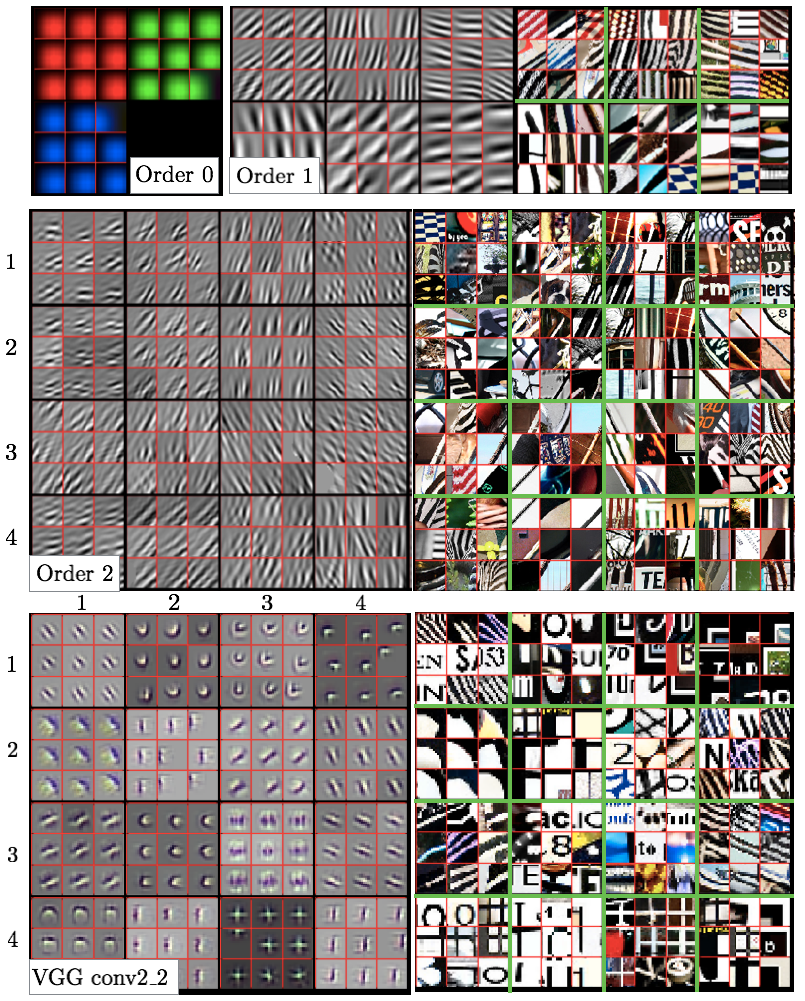
\includegraphics[width=1.1\textwidth]{images/deconv_images.png}}
      \caption[Visualization of deconvolved features]
              {Visualization of some deconvolved features.  9 coordinates are chosen in the
              feature map for layer 1 $z^1$, 16 for the second layer
              feature map $z^2$ and 16 for the third layer feature map.
              The entire dataset is run, and 9 images that made the largest
              activation at this point are noted. Deconvolution is then done on
              the feature maps from these 9 images, and the results are shown
              next to the actual images. Deeper layers are picking up more
              complex structures. Taken from \citep{zeiler_visualizing_2014}.}
  \end{figure}

  \citeauthor{mahendran_understanding_2015} take a slightly different route on
  deconvolution networks \citep{mahendran_understanding_2015}. They do not
  store this extra information but instead define a cost function to maximize
  to. This results in visualization images that look very surreal, and can be
  quite different from the input.

\section{Introduction}
\label{sec:intro}
Scattering transforms, or ScatterNets, have recently gained much attention and
use due to their ability to extract generic and descriptive features in well
defined way. They can be used as unsupervised feature extractors
for image classification \cite{bruna_invariant_2013, oyallon_deep_2015, 
singh_dual-tree_2017, singh_multi-resolution_2017} and texture classification
\cite{sifre_rotation_2013}, or in combination with supervised methods such as
Convolutional Neural Networks (CNNs) to make the latter learn quicker, and in
a more stable way \cite{oyallon_scaling_2017}. 

ScatterNets have been shown to perform very well as image classifiers. In
particular, they can outperform CNNs for classification tasks with reduced
training set sizes, e.g.\ in CIFAR-10 and CIFAR-100 (Table 6 from
\cite{oyallon_scaling_2017} and Table 4 from \cite{singh_dual-tree_2017}).  
They are also near state-of-the-art for Texture Discrimination tasks
(Tables 1--3 from \cite{sifre_rotation_2013}). Despite this, there still exists
a considerable gap between them and CNNs on challenges like CIFAR-10 with the
full training set ($~83\%$ vs.\ $~93\%$). Even considering the benefits of
ScatterNets, this gap must be addressed.

We first revise the operations that form a ScatterNet in
\autoref{sec:scatternet}. We then introduce our DeScatterNet
(\autoref{sec:descatternet}), and show how we can use it to examine the layers of ScatterNets
(using a similar technique to the CNN visualization in
\cite{zeiler_visualizing_2014}). We use this analysis tool to
highlight what patterns a ScatterNet is sensitive to
(\autoref{sec:visualization}), showing that they are very
different from what their CNN counterparts are sensitive to, and possibly less
useful for discriminative tasks. 

We use these observations to propose an architectural change to ScatterNets,
which have not changed much since their inception in \cite{mallat_group_2012}. 
Two changes of note however are the work of Sifre and Mallat in
\cite{sifre_rotation_2013}, and the work of Singh and Kingsbury in
\cite{singh_dual-tree_2017}.  Sifre and Mallat introduced Rotationally Invariant
ScatterNets which took ScatterNets in a new direction, as the architecture now
included filtering across the wavelet orientations (albeit with heavy
restrictions on the fitlers used).  Singh and Kingsbury achieved improvements in
performance in a Scattering system using the spatially implementable \DTCWT
\cite{kingsbury_complex_2001} wavelets instead of the Fourier Transform (FFT)
based Morlet previously used.

We build on these two systems, showing that with carefully designed complex
filters applied across the complex spatial coefficients of a 2-D \DTCWT,  
we can build filters that are sensitive to more recognizable shapes like
those commonly seen in CNNs, such as corners and curves (\autoref{sec:corners}). 

\section{The Scattering Transform}
\label{sec:scatternet}
% These have two distinct advantages and one
% disadvantage over the Fourier based implementation:
% \begin{itemize}
  % \pro They are implemented directly with spatially separable convolutions. This
  % gives direct access to the wavelet coefficients (much in the same way as we
  % have direct access to the activations in a CNN), rather than having to
  % take transforms and inverse transforms to do an efficient convolution. This
  % also opens them up far more easily to be modifiable with an algorithm like
  % backpropagation. 
  % % \emph{is it easy to backpropagate through a forward and
  % % backward FFT? They are linear operations, but not sure how well it will
  % % work}.
  % % \pro ??? The \DTCWT wavelets form a Parseval tight-frame, making them energy
  % % preserving.
  % \pro Can efficiently handle any sized input (useful for fully convolutional
  % nets) as we do not need to pre compute filter FFTs.
  % \con They are restricted to 6 orientations, whereas the Morlet wavelets are
  % free to have a variable number. In practice however, it seems that the number
  % of orientations does not vary much, and a good number is around 8.
% \end{itemize}
% Acknowledging that there will be a subtle difference between our implementation
% and the one in \cite{oyallon_deep_2015}, we shift our focus now to what is
% similar between the two. 

% \begin{figure*}[ht]
  % \centering
  % \includegraphics[width=\textwidth]{scatnet_blk.jpeg}
  % \caption{Three layer Scatternet figure, included as a visual aid for}
  % \label{fig:scat}
% \end{figure*}
The Scattering Transform, or ScatterNet, is a cascade of complex wavelet transforms and
modulus non-linearities (throwing away the phase of the complex wavelet
coefficients). At a chosen scale, averaging filters provide invariance
to nuisance variations such as shift and deformation (and potentially
rotations). Due to the non-expansive nature of the wavelet
transform and the modulus operation, this transform is stable to
deformations. 

Typical implementations of the ScatterNet are limited to two `orders'
(equivalent to layers in a CNN) \cite{oyallon_deep_2015, singh_dual-tree_2017,
oyallon_scaling_2017}. In addition to scattering \emph{order}, we also have the
\emph{scale} of invariance, $J$. This is the number of band-pass coefficients
output from a wavelet filter bank (FB), and defines the cut-off frequency for
the final low-pass output: $2^{-J}\frac{f_s}{2}$ ($f_s$ is the sampling
frequency of the signal). Finally, we call the number of oriented wavelet
coefficients used $L$.  These are the three main hyper-parameters of the
scattering transform and must be set ahead of time. We describe a system with
scale parameter $J=4$, order $m=2$ and with $L=6$ orientations ($L$ is fixed
to 6 for the \DTCWT but is flexible for the FFT based Morlet wavelets).

Consider an input signal $x(\bm{u}), \bm{u}\in\reals[2]$. The zeroth order
\textbf{scatter} coefficient is the lowpass output of a $J$ level FB: 

\begin{equation}
  S_0x(\bm{u}) \definedas (x \conv \phi_J)(\bm{u})
\end{equation}

This is invariant to translations of up to $2^J$ pixels\footnote{From here on,
we drop the $\bm{u}$ notation when indexing $x$, for clarity.}. In exchange for
gaining invariance, the $S_0$ coefficients have lost a lot of information
(contained in the rest of the frequency space). The remaining energy of $x$ is
contained within the first order \textbf{wavelet} coefficients:

\begin{equation}
W_1x(\bm{u}, j_1, \theta_1) \definedas x \conv \psi_{j_1, \theta_1}
\end{equation}

for $j_1\in\{1,2, \ldots, J\}, \theta_1\in\{1,2, \ldots, L\}$. We will want to
retain this information in these coefficients to build a useful classifier.

Let us call the set
of available scales and orientations $\Lambda_1$ and use $\lambda_1$ to index it.
For both Morlet and \DTCWT\ implementations, $\psi$ is complex-valued, i.e.,
$\psi = \psi^r + j\psi^i$ with $\psi_r$ and $\psi_i$ forming a Hilbert Pair,
resulting in an analytic $\psi$.
 This analyticity provides a source of
invariance --- small input shifts in $x$ result in a phase rotation (but little
magnitude change) of the complex wavelet coefficients\footnote{In comparison to
a system with purely real filters such as a CNN, which would have rapidly
varying coefficients for small input shifts \cite{kingsbury_complex_2001}.}.

Taking the magnitude of $W_1$ gives us the first order \textbf{propagated}
signals:

\begin{equation}
  U_1x(\bm{u}, \lambda_1) \definedas |x\conv \psi_{\lambda}| 
    = \sqrt{(x \conv \psi^r_{\lambda_1})^2 + (x \conv \psi^i_{\lambda_1})^2}
\end{equation}

The first order scattering coefficient makes $U_1$ invariant up to our
scale $J$ by averaging it:

\begin{equation}
  S_1x(\bm{u}, \lambda_1) \definedas |x\conv \psi_{\lambda}| \conv \phi_J
\end{equation}

If we define $U_0 \definedas x$, then we can iteratively define:

\begin{eqnarray}
  W_{m} &=& U_{m-1} \conv \psi_{\lambda_{m}} \\
  U_{m} &=& |W_{m}| \\
  S_{m} &=& U_m \conv \phi_J
\end{eqnarray}

We repeat this for higher orders, although previous work shows that, for natural
images, we get diminishing returns after $m=2$. The output of our ScatterNet is
then:

\begin{equation}
  Sx = \{S_0x, S_1x, S_2x\}
\end{equation}
% The set of coefficients $\{S_0x, W_1x\}$ will have the same energy as $x$
% (due to the tight frame nature of the wavelets). As the modulus operator is
% energy preserving, then $\{S_0x, U_1x\}$ 
% must also have the same energy as $x$. However, we lose some energy going from
% $U_1x$ to $S_1x$ due to the low-pass filtering. We retain this lost energy in
% the second order coefficients
% by adding in band-pass filters: 
% $$  U_2(\bm{u}, \lambda_1, \lambda_2) =  ||x \conv \psi_{\lambda_1}| \conv
    % \psi_{\lambda_2}| $$
% and again, we can make these invariant by averaging over a scale $J$
% $$ S_2(\bm{u}, \lambda_1, \lambda_2) = ||x \conv \psi_{\lambda_1}| \conv
    % \psi_{\lambda_2}| \conv \phi_J $$
% Note that the set  $\Lambda_2$ indexed by $\lambda_2 = (j_2, \theta_2)$ is
% a strict subset of $\Lambda_1$. We only compute increasing paths $j_2 > j_1$, as
% non-increasing paths have no energy \cite{bruna_invariant_2013}.  Again, the set
% of coefficients $\{S_0x, S_1x, U_2x\}$ will have the same energy as $x$,
% but $\{S_0x, S_1x, S_2x\}$ will have slightly less. 

\subsection{Scattering Color Images}
A wavelet transform like the \DTCWT\ accepts single channel input, while we
often work on RGB images. This leaves us with a choice. We can either:
\begin{enumerate}
  \item Apply the wavelet transform (and the subsequent scattering operations)
    on each channel independently. This would triple the output size to $3C$.
  \item Define a frequency threshold below which we keep color information, and
    above which, we combine the three channels into a single luminance channel.
\end{enumerate}
The second option uses the well known fact that the human eye is far less sensitive 
to higher spatial frequencies in color channels than in luminance channels. 
This also fits in with the first layer filters seen in the well known
Convolutional Neural Network, AlexNet. Roughly one half of the filters were low
frequency color `blobs', while the other half were higher frequency, grayscale,
oriented wavelets. 

For this reason, we choose the second option for the
architecture described in this paper. We keep the 3 color
channels in our $S_0$ coefficients, but work only on grayscale for high orders 
(the $S_0$ coefficients are the lowpass bands of a J-scale wavelet transform, so
we have effectively chosen a color cut-off frequency of $2^{-J} \frac{f_s}{2}$).

For example, consider an RGB input image $x$ of size $64\x 64\x 3$. The 
scattering transform we have described with parameters $J=4$ and $m=2$ would
then have the following coefficients:
% \footnote{we have oversampled the outputs by
% a factor of 2, as in \cite{oyallon_deep_2015, singh_dual-tree_2017}}.
\begin{eqnarray*}
  S_0 &:& (64\x 2^{-J}) \x (64\x 2^{-J}) \x 3 = 4\x 4\x 3 \\
  S_1 &:& 4\x 4\x (L J) = 4\x 4\x 24 \\
  S_2 &:& 4\x 4\x \left(\frac{1}{2}L^2 J(J-1)\right) = 4\x 4\x 216 \\
  S &:& 4\x 4\x (216+24+3) = 4\x 4\x 243
\end{eqnarray*}

\section{The Inverse Network}
% \vspace{-5}
\label{sec:descatternet}
\begin{figure*}[ht]
  \centering
  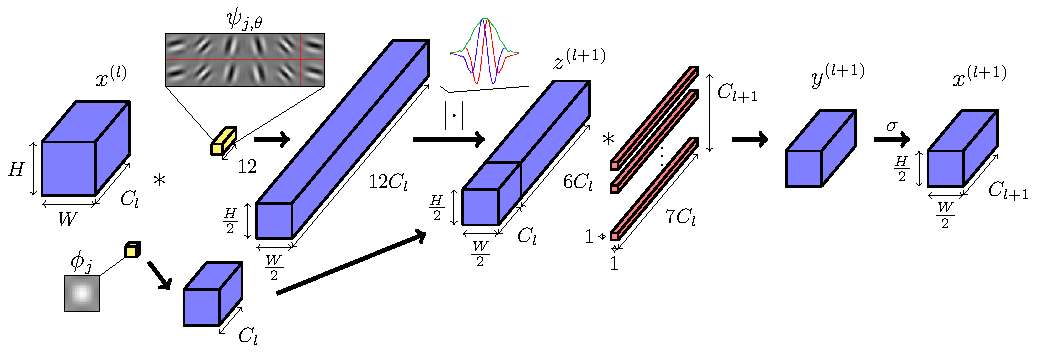
\includegraphics[width=\textwidth]{figure1.png}
  \caption{A DeScattering layer (left) attached to a Scattering layer (right).
  We are using the same convention as \cite{zeiler_visualizing_2014}
  Figure 1 - the input signal starts in the bottom right hand corner, passes
  forwards through the ScatterNet (up the right half), and then is 
  reconstructed in the DeScatterNet (downwards on the left half).
  The DeScattering layer will reconstruct an approximate version of the previous
  order's propagated signal. The $2\x 2$ grids shown around the image are either Argand
  diagrams representing the magnitude and phase of small regions of
  \emph{complex} (De)ScatterNet
  coefficients, or bar charts showing the magnitude of the \emph{real}
  (De)ScatterNet coefficients (after applying the modulus non-linearity). For reconstruction, we
  need to save the discarded phase information and reintroduce it by multiplying
  it with the reconstructed magnitudes.}
  \label{fig:descat}
\end{figure*}
\label{sec:invscat}
We now introduce our inverse scattering network. This allows us to back project
scattering coefficients to the image plane; it is inspired by the
\textbf{DeconvNet} used by Zeiler and Fergus in
\cite{zeiler_visualizing_2014} to look into the deeper layers of CNNs. 

We emphasize that instead of thinking about perfectly reconstructing $x$ from
$S\in \reals[H'\x W'\x C]$, we want to see what signal/pattern in the input image caused
a large activation in each channel. This gives us a good idea of what each
output channel is sensitive to, or what it extracts from the input. 
Note that we do not use any of the log normalization layers described in
\cite{oyallon_deep_2015, singh_dual-tree_2017}.


\subsection{Inverting the Low-Pass Filtering}
Going from the $U$ coefficients to the $S$ coefficients involved convolving by
a low pass filter, $\phi_J$ followed by decimation to make the output $(H\x
2^{-J})\x (W\x2^{-J})$.  $\phi_J$ is a purely real filter, and we can `invert'
this operation by interpolating $S$ to the same spatial size as $U$ and convolving with
the mirror image of $\phi_J$, $\widetilde{\phi}_J$ (this is equivalent to the
transpose convolution described in \cite{zeiler_visualizing_2014}). 

\begin{equation}
  \label{eq:s_hat}
  \hat{S}_{m} = S_{m} \conv \widetilde{\phi}_J
\end{equation}

This will not recover $U$ as it was on the forward pass, but will recover all
the information in $U$ that caused a strong response in $S$.

\subsection{Inverting the Magnitude Operation}
In the same vein as \cite{zeiler_visualizing_2014}, we face a difficult
task in inverting the non-linearity in our system. 
% It has been proven that for
% particular wavelets, we can recover the phase from their modulus
% \cite{waldspurger_phase_2012}, but this is not a trivial operation. Instead, we
We lend inspiration from the \emph{switches} introduced in the DeconvNet; the
switches in a DeconvNet save the location of maximal activations so that
on the backwards pass activation layers could be unpooled trivially. We do an
equivalent operation by saving the phase of the complex activations. On the
backwards pass we reinsert the phase to give our recovered $W$.
\begin{equation}
  \label{eq:w_hat}
  \hat{W}_{m} = \hat{U}_{m}e^{j\theta_{m}}
\end{equation}

\subsection{Inverting the Wavelet Decomposition}
Using the \DTCWT makes inverting the wavelet transform simple, as we
can simply feed the coefficients through the synthesis filter banks to regenerate
the signal. For complex $\psi$, this is convolving with the conjugate transpose
$\widetilde{\psi}$: 

\begin{eqnarray}
  \label{eq:x_hat}
  \hat{U}_{m-1} &=& \hat{S}_{m-1} + \hat{W}_{m} \nonumber \\
              &=& S_{m-1} \conv \widetilde{\phi}_J + \sum_{j, \theta} W_{m}(\bm{u}, j,
  \theta) \conv \widetilde{\psi}_{j, \theta}
\end{eqnarray}

\begin{figure*}[htp]
  \centering
  \includegraphics[width=0.9\textwidth]{figure2.png}
  \caption{Visualization of a random subset of features from $S_0$ (all
  3), $S_1$ (6 from the 24) and $S_2$ (16 from the 240) scattering
    outputs. We record the top 9 activations for the chosen features and project
    them back to the pixel space. We show them alongside the input image patches
    which caused the large activations. We also include reconstructions from
    layer conv2\_2 of VGG Net \cite{simonyan_very_2014}(a popular CNN, often used
    for feature extraction) for reference --- here we display 16 of the 128
    channels. The VGG reconstructions were made with a CNN DeconvNet based on
    \cite{zeiler_visualizing_2014}. Image best viewed digitally.}
  \label{fig:reconstructions}
\end{figure*}
\begin{figure*}[t]
  \centering
  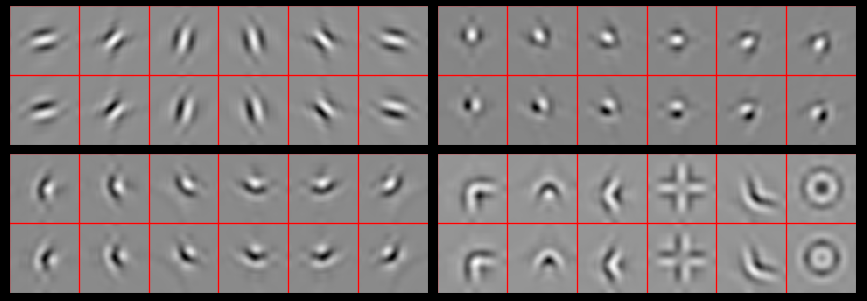
\includegraphics[width=0.9\textwidth]{figure3.png}
  \caption{Shapes possible by filtering across the wavelet orientations with
  complex coefficients. All shapes are shown
  in pairs: the top image is reconstructed from a purely real output, and the
  bottom image from a purely imaginary output. These `real' and `imaginary' shapes 
  are nearly orthogonal in the pixel space (normalized dot product $<0.01$ for
  all but the doughnut shape in the bottom right, which has $0.15$) but produce
  the same $U'$, something that would not be possible without the complex
  filters of a ScatterNet.  Top left - reconstructions from $U_1$ (i.e.\ no
  cross-orientation filtering). Top right- reconstructions from $U_1'$ using
  a $1\x 1\x 12$ Morlet Wavelet, similar to what was done in the `Roto-Translation'
  ScatterNet described in \cite{sifre_rotation_2013, oyallon_deep_2015}. Bottom
  left - reconstructions from $U_1'$ made with a more general $1\x 1\x 12$
  filter, described in \autoref{eq:simple_corner}. Bottom
  right - some reconstructions possible by filtering a general $3\x 3\x 12$ filter. }
  \label{fig:newshapes}
\end{figure*}

\section{Visualization with Inverse Scattering}
\label{sec:visualization}

To examine our ScatterNet, we scatter all of the images from ImageNet's validation
set and record the top 9 images which most highly activate each of the $C$
channels in the ScatterNet. This is the \emph{identification} phase (in which no
inverse scattering is performed). 

Then, in the \emph{reconstruction}
phase, we load in the $9\x C$ images, and scatter them one by one. We take the
resulting $4\x 4\x 243$ output vector and mask all but a single value in the channel we are currently examining.

This 1-sparse tensor is then presented to the inverse scattering network from
\autoref{fig:descat} and projected back to the image space. Some results of this
are shown in \autoref{fig:reconstructions}. This figure shows reconstructed
features from the layers of a ScatterNet. For a given output channel, we show
the top 9 activations projected independently to pixel space. For the first and
second order coefficients, we also show the patch of pixels in the input image
which cause this large output. We display activations from various scales
(increasing from first row to last row), and random orientations in these
scales. 

The order 1 scattering (labelled with `Order 1' in
\autoref{fig:reconstructions}) coefficients look quite similar to the first
layer filters from the well known AlexNet CNN \cite{krizhevsky_imagenet_2012}.
This is not too surprising, as the first order scattering coefficients are
simply a wavelet transform followed by average pooling. They are responding to
images with strong edges aligned with the wavelet orientation. 

The second order coefficients (labelled with `Order
2' in \autoref{fig:reconstructions}) appear very similar to the order
1 coefficients at first glance.
They too are sensitive to edge-like features, and some of them (e.g.\ third row,
third column and fourth row, second column) are mostly just that. These are
features that have the same oriented wavelet applied at both the first and
second order.  Others, such as the 9 in the first row, first column, and first
row, fourth column are more sensitive to checker-board like patterns. Indeed,
these are activations where the orientation of the wavelet for the first and
second order scattering were far from each other (15\degs and 105\degs for the
first row, first column and 105\degs and 45\degs for the first row, fourth
column).

For comparison, we include reconstructions from the second layer of the
well-known VGG CNN\@ (labelled with `VGG conv2\_2', in
\autoref{fig:reconstructions}). These were made with a DeconvNet, following the
same method as \cite{zeiler_visualizing_2014}. Note that while some of
the features are edge-like, we also see higher order shapes like corners,
crosses and curves.
% \vspace{-5pt}

\section{Corners, Crosses and Curves}
\label{sec:corners}
% The work in \cite{oyallon_deep_2015} demonstrated that second order scattering
% coefficients are necessary, and give a large increase in accuracy over using
% just the first order coefficients.
These reconstructions show that the features extracted from ScatterNets vary
significantly from those learned in CNNs after the first order. In many
respects, the features extracted from a CNN like VGGNet look preferable for use
as part of a classification system.
% We now propose an additional layer that can be added to our
% ScatterNet with ease, which generates filters sensitive to these higher order
% shapes. In fact, we have a great deal of flexibility with what shapes we can be
% sensitive to.

\cite{sifre_rotation_2013} and \cite{oyallon_deep_2015} introduced the idea of
a `Roto-Translation' ScatterNet. Invariance to rotation could be made by
applying averaging (and bandpass) filters across the $L$ orientations 
from the wavelet transform \emph{before} applying the complex modulus.
Momentarily ignoring the form of the filters they apply, referring to them
as $F_k\in \complexes[L]$, we can think of this stage as stacking the $L$
outputs of a complex wavelet transform on top of each other, and convolving
these filters $F_k$ over all spatial locations of the wavelet coefficients $W_m
x$ (this is equivalent to how filters in a CNN are fully connected
in depth):

\begin{equation}
  V_m x(\bm{u}, j, k) = W_{m}x \conv F_k = \sum_{\theta} W_{m}x(\bm{u}, j, \theta)
F_k(\theta)
\end{equation}

We then take the modulus of these complex outputs to make a second propagated
signal:

% \vspace{-10pt}
\begin{equation}
  U_{m}'x \definedas |V_{m}x| = |W_{m}x \conv F_k| = |U_{m-1}x
  \conv \psi_{\lambda_{m}} \conv F_k|
\end{equation}

We present a variation on this idea, by filtering with a more general 
$F\in \complexes[H\x W\x 12]$. We use $F$ of length 12 rather than 6, as we use
the $L=6$ orientations and their complex conjugates; each wavelet is a 30\degs
rotation of the previous, so with 12 rotations, we can cover the full
$360\degs$. 
% The filters can be shared across scales J to produce the same shapes at
% different scales. Further, if $F\in \complexes[1\x 1\x 12]$, then we can 
% create 12 orientations of the same shape by simply rotating the
% filter coefficients in $F$ by one sample along the third dimension; each sample
% shift rotating the shape by $30\degs$. For more general shaped $F$, we can still
% trivially get rotations of the shape, but it requires rotating the coefficients
% spatially too.

\autoref{fig:newshapes} shows some reconstructions from these $V$ coefficients.
Each of the four quadrants show reconstructions from a different class of
ScatterNet layer. 
All shapes are shown in real and imaginary Hilbert-like pairs; the top images in
each quadrant are reconstructed from a purely real $V$, while the bottom inputs
are reconstructed from a purely imaginary $V$. This shows one level of invariance of
these filters, as after taking the complex magnitude, both the top and the
bottom shape will activate the filter with the same strength. In comparison, for
the purely real filters of a CNN, the top shape would cause a large output, and
the bottom shape would cause near 0 activity (they are nearly orthogonal to each
other).

In the top left, we display the 6 wavelet filters for reference (these were
reconstructed from $U_1$, not $V_1$). In the top right of the figure we see some
of the shapes made by using the $F$'s from the Roto-Translation ScatterNet
\cite{sifre_rotation_2013, oyallon_deep_2015}.  The bottom left is where we
present some of our novel kernels. These are simple corner-like shapes made 
by filtering with ${F\in \complexes[1\x 1\x 12]}$
% \vspace{-10pt}
\begin{equation}
\label{eq:simple_corner}
F = [1, j, j, 1, 0, 0, 0, 0, 0, 0, 0, 0]
\end{equation}
The six orientations are made by rolling the coefficients in $F$ along one
sample (i.e. $[0, 1, j, j, 1, 0,\ldots]$, $[0,0,1,j,j,1,0,\ldots]$,
$[0,0,0,1,j,j,1,0, \ldots]$ \ldots). Coefficients roll back around (like
circular convolution) when they reach the end.

Finally, in the bottom right we see shapes made by 
${F \in \complexes[3\x 3\x 12]}$. Note that with the exception of the 
ring-like shape which has 12 non-zero coefficients, all of these shapes were
reconstructed with $F$'s that have 4 to 8 non-zero coefficients of a possible 
64. These shapes are now beginning to more closely resemble the more complex
shapes seen in the middle stages of CNNs. 

% \vspace{-5pt}
\section{Discussion}
This paper presents a way to investigate what the higher orders of a ScatterNet
are responding to - the DeScatterNet described in \autoref{sec:descatternet}.
Using this, we have shown that the second `layer' of a ScatterNet 
responds strongly to patterns that are very dissimilar to those that highly activate the
second layer of a CNN\@. As well as being dissimilar to CNNs, visual inspection of the
ScatterNet's patterns reveal that they may be less useful for discriminative
tasks, and we believe this may be causing the current gaps in state-of-the-art
performance between the two. 

We have presented an architectural change to ScatterNets that can make it
sensitive to more recognizable shapes. We believe that using this new layer is
how we can start to close the gap, making more generic and descriptive
ScatterNets while keeping control of their desirable properties. 

A future paper will include classifier results for these new filters.

% \pagebreak
% References should be produced using the bibtex program from suitable
% BiBTeX files (here: strings, refs, manuals). The IEEEbib.bst bibliography
% style file from IEEE produces unsorted bibliography list.
% -------------------------------------------------------------------------
\bibliographystyle{IEEEbib}
